\subsubsection{Introduction}
%LET'S GO TEAM!!! ONE LESS SECTION
%We are unstoppppable --> DAB DAB DAB
In this part of the chapter the orbital is studied using the model of special perturbations, which as previously defined, is the one that uses a numerical step-by-step integration. There are three manly used methods to study the dynamic propagation of an orbit, which are:\\

\paragraph{Cowell's method} This is the simplest method since it does not require any assumption or approximation. It is based on quantifying the accelerations produced by the perturbations and adding them to the dynamic equation of a Keplerian orbit (see Orbit Design: Chapter 1 equation 1.2.3) leading to:

\begin{equation}\label{eq:ode}
\frac{d^2 \vec{r}}{d t^2}=-\frac{\mu}{r^3}\vec{r}+\vec{a}_p
\end{equation}

Where $\vec{a}_p$ is the acceleration produced by the perturbations. This second order differential equation is the one that must be integrated in order to propagate the orbit. Although the formulas and application of this method are simple, this does not imply that it lacks robustness or precision. Its results are as good as any of the following two methods but the major drawback of \textit{Cowell's method} is that it requires smaller time-steps being therefore slower (in terms of computation speed).

\textbf{Encke's Method:} This method is based on correcting the defects of the previous method. Encke uses a schema based on what is called \textit{predictor-corrector}. First, it evaluates the orbit as if it were a Keplerian orbit (i.e. without perturbations) and then it integrates only the perturbations to correct the deviation caused by considering the unperturbed orbit. Its advantage over Cowell's method is clear, since it only integrates perturbations, and since these vary less over time than the position itself, we can relax the integration by increasing the time step. In short, this scheme is faster but also more complex to program than the one proposed by Cowell.

\textbf{Variation of the parameters:} This method, developed by Lagrange, is based on considering the orbit as a succession of Keplerian orbits, each of them being tangent to the satellite orbit at a certain point. Thus we can obtain differential equations that model the variation of the orbital parameters as a function of time.

The formulations and schemes followed by each of these methods can be found in any reference dealing with orbital mechanics. For example, the reader can refer to \cite{Vallado2007} or the chapter 20 of \cite{Bate1971} to obtain more detailed information about these methods.

For the purposes of this study, implementing the simplest method is enough. As it has already mentioned, it is based on adding the perturbations (discussed at the beginning of this chapter) to the dynamics equation. A \emph{Matlab} routine has been developed that follows the next scheme:

\begin{figure}[H]
\centering
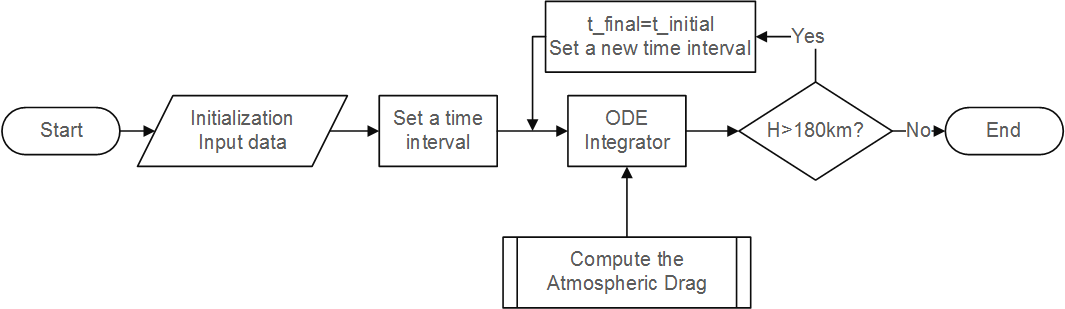
\includegraphics[scale=.7]{./decay/Diagram.png}
\caption{Algorithm of resolution used to solve the orbital propagation.}
\end{figure}

The disturbances that the routine includes are:

\begin{itemize}
\item The potential field of the earth.
\item The Atmospheric drag.
\item The influences of 3 bodies.
\item Solar Radiation Pressure.
\end{itemize}

As it has been seen in previous sections, the only truly significant perturbation for the orbital decay at the altitude in which the constellation is located is the one caused by the atmospheric drag. Thus, other contributions have been deactivated to speed up the calculation. Therefore, explaining the formulation used to obtain the accelerations caused by these perturbations is not of interest for the development of the study. However, the following are the sources from which they were obtained:

\begin{itemize}
\item The calculation of the Earth gravity Potential uses the equation~\ref{eq:Oblat}. Following the indications of \cite{Bate1971} both the Legendre polynomials and the parameters $C _{nm}$ and $S _{nm}$ can be obtained.

\item The equations present in \cite{Junkins} have been used to compute the perturbations due to other bodies,  

\item For Solar Radiation pressure the formulation used is the one presented in\cite{Kufa} including a 'shadow factor' (if the earth is between the sun and the satellite, the latter will not receive direct radiation from the Sun) modelled by a normal statistical distribution.

\item For the calculation of Drag, the equation \ref{eq:drag} and the atmosphere model presented in the same section have been used.
\end{itemize}


To be able to integrate the system we must take into account that, in fact, as we work in Cartesian coordinates, it is a system of three equations. Moreover, since it is a second-order equation we must rewrite it as a first-order system. Let $x_1=r=(x, y, z)$ and $x_2=\dot{x}_1=\dot{r}=(vx, vy, vz)$. Therefore:

\begin{equation}
X=
\begin{pmatrix}
 x\\ 
 y\\ 
 z\\ 
 v_x\\ 
 v_y\\ 
 v_z\\  
 \end{pmatrix}
\Rightarrow
\dot{X}=
\begin{pmatrix}
 v_x\\ 
 v_y\\ 
 v_z\\  
\ddot{x}\\ 
\ddot{y}\\ 
\ddot{z}\\  
 \end{pmatrix}
=
\begin{pmatrix}
 v_x\\ 
 v_y\\ 
 v_z\\  
 a_{p,x}-\frac{\mu}{r^3}x\\ 
 a_{p,y}-\frac{\mu}{r^3}y\\ 
 a_{p,z}-\frac{\mu}{r^3}z\\  
 \end{pmatrix}
\end{equation}

To integrate this system, you can use the \emph{Matlab} built-in function \textbf{ode45}, which is a runge-kutta 4-5 with a variable step control that basically modifies the time step if the error is too large.
Also, the \textbf{juliandate.m} function (included in the Matlab Aerospace module) have been used. It calculates the Julian Date,that is the number of days since noon Universal Time on January 1, 4713 ECB ( On the Julian calendar).

\subsubsection{Results}
A simulation has been executed with the same parameters as in the previous section. After 932 seconds of computation, the results obtained are shown below:

\begin{figure}[H]
\centering
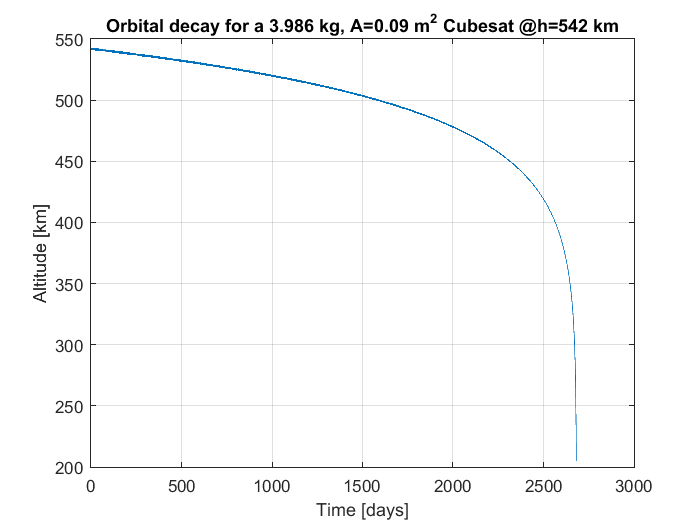
\includegraphics[scale=1]{./decay/graph.png}
\caption{Orbital decay of the satellite.}
\label{fig:COE}
\end{figure}

As it can be seen, the estimated orbital decay for a satellite like Astrea's Cubesat is about 2700 days or, what is the same, 7.4 years. This estimation and the temporal evolution of the altitude is in agreement with the results obtained by the semi-analytic method. It is therefore verified that for a preliminary analysis and the respective modifications that it can present (i.e. changes in weight, changes in area, initial height, geometry of the orbit) it is enough with the results obtained by the semi-analytic study, which do not require almost computation time (only a few seconds), avoiding the expense of computing resources that would produce a dynamic simulation for every modification.